\documentclass[]{article}

% Packages

% Pseudocode
\usepackage{algpseudocode}
\usepackage{algorithm}

% Placing
\usepackage{float}
% Drawing
\usepackage{tikz}
% Memory maps
\usepackage{bytefield}
% Simple trees
\usepackage{qtree}
% Custom colors
\usepackage{xcolor}
% Comments
\usepackage{verbatim}
% math symbols
\usepackage{amssymb}

% Plots
\usepackage{pgfplots}
\pgfplotsset{compat = newest}

% Dependencies
\usepackage{mymacros}
\usepackage{parallelP}


% Title
\title{Orthogonal Recursive Bisection on the GPU for Accelerated Load Balancing in Large N-Body Simulations \\ - \\ Bachelor Thesis}

\author{Andrin Rehmann}

% Start
\begin{document}

\maketitle

\newpage

\tableofcontents

\newpage
\section{Introduction}


The N-Body technique has been used for decades to simulate the Universe so we can compare theory with observations. This technique uses ``particles'' or ``bodies'' to sample phase space, and as gravity operates over infinite distance it is necessary to consider all pair-wise interactions which makes a naive implementation $\mathcal{O}(n^2)$.
It is clear that this does not scale particularly well with large particle counts.

One common approach is to decompose the particles into a tree structure and multipole expansions of the particles in each tree cell to approximate the forces. This reduces the complexity of the algorithm to $\mathcal{O}(n\log{}n)$. More recently the Fast Multipole Method (FMM) has gained wider option primarily due to the extremely large sizes of modern simulations. This technique further reduces the complexity to $\mathcal{O}(n)$!

The computational effort required in modern N-Body simulations can thus be split into three categories:

\begin{itemize}
	\item \textbf{Load Balancing:} Distribute particles equally among nodes with regards to memory.
	\item \textbf{Tree Building:} Build tree on each node for accelerated force calculation and integration.
	\item \textbf{Force calculation and integration:} Calculate forces between particles and apply them.
\end{itemize}

Before the implementation of FMM into codes, and particularly before the era of modern accelerated computing (e.g., SIMD vectorization and GPU computing) the forces calculations dominated the computational cost. In more recent simulations, each category is about one third of the total calculation time\cite{2017ComAC...4....2P}. This makes the tree building and load balancing subjects to great performance gains, since GPU acceleration is usually not exploited. 

This project proposes to implement Tree Building with the GPU using CUDA to accelerate load balancing.

\subsection{Target Data}\label{section:target-data}

\TODO{Write about properties of datasets}

The target data consists of $N$ particles where each particle has several data points and introduce the following definitions:

\begin{itemize}
	\item We define a particle as $p_i$  where $i \in \{0,...,N\}$. 
	\item We define the space of binary numbers with a precision of $p$ as $\mathbb{B}_p$ where we have $a \in \mathbb{B}_p \Leftrightarrow a \in \{0,1\}^{p}$
	\item We define the corner coordinates of the boundary box with $\vec{lower}, \vec{upper}$ where we have $\vec{b} \in \mathbb{B}_p^3$. 
	\item We define the coordinates of a particle $p_i$ as $\vec{x_i}$ for which holds $\{\vec{x} | \vec{lower} \leq \vec{x} \leq \vec{upper}, \vec{x} \in \mathbb{B}_p^3 \}$.

\end{itemize}

\begin{figure}[H]
	\begin{center}
		\begin{tikzpicture}
			\randistr{10}{5}{100}
			\draw (0,0) rectangle (10, 5);
			\filldraw  (0,0) circle (3pt) node [anchor=west]{};
			\node[yshift=0.3cm, xshift=-0.3cm] at (0,0) {$-\frac{b}{2}$};
			
			\filldraw  (10,5) circle (3pt) node [anchor=west]{};
			\node[yshift=0.3cm, xshift=-0.3cm] at (10,5) {$\frac{b}{2}$};
		\end{tikzpicture}
	\end{center}
\caption{Unfiorm random distribution of 3D coordinates in square domain projected onto a 2d plane}
\end{figure}

\Q{Ask Doug}

\subsection{Force Integration and FFM}\label{section:force-integration}

\TODO{Write about how the very unequal data can also affect integration }
Non equal weighting functions for different particles are due to higher accelerations and greater proximity to strong gravitational influences. This in turn requires a higher integrations accuracy to mitigate errors. When we try to balance the workload, this implies drawbacks in terms of memory balance. 



\subsection{Target Computing Systems}\label{section:target-systems}

\TODO{Write about systems which can be used to test data and systems which are worth considering while estimating runtimes of this approach.}

\subsection{PKDGrav}

\TODO{Brief summary of PKDGrav and how this work can be used to improve PKDGrav}

\newpage
\section{Orthogonal Recursive Bisection (ORB)}


%https://de.overleaf.com/learn/latex/TikZ_package
%https://texample.net/tikz/examples/
In this section we will introduce the ORB algorithm along with subroutines. We will use the concept of binary trees and in order to have clear understanding of steps of the algorithm, we will use the following terminologies: 

\begin{itemize}
	\begin{comment}
		\item The left child of a node with index $i$ has the index $2\times i$. 
	\item The right child of a node with index $i$ has the index $i*2 + 1$. 
	\item The parent of a node with index $i$ has the index $\lfloor \frac{i}{2} \rfloor$. 
	\item The root node has the index $i$.
	\end{comment}

	\item The domain of a node is the area it compasses. 
\end{itemize}


In principle the ORB Algorithm is used to partition a multi dimensional domain into subdomains based on spatial proximity. It does so by splitting a $k$ dimensional domain containing $N$ particles into $d$  subdomains each of $k$ dimensions. This is most efficiently achieved using a recursive algorithm. During the recursive process, we store all intermediate domains a binary tree. We can leverage the resulting binary in two ways:

\begin{enumerate}
	\item For simulation code and more specifically for the Fast Multipole Method the tree can be leveraged to greatly accelerate the simulation time. \TODO{expand}
	\item The tree can be used to equally distribute memory and/or workload among nodes or processors in a computing system. 
\end{enumerate} 

Our main objective in this work is to improve the runtime of astrophysical simulations, or more specifically PKDGrav. At the same time we want to minimize penalties in regards to $N$, the total number of particles, such that we can leverage a high $N$ to increase the precision of the simulation. Furthermore we want to adapt and optimize the algorithms with regards to the target data as introduced in \ref{section:target-data} and target computing systems (\ref{section:target-systems}).

\subsection{Memory and Workload Balancing}\label{sec:balancing}
We have now formulated our main objectives for improving ORB, which are to improve the runtime but at the same time keeping $N$ as large as possible. In this section we will explain how the two cannot be maximized at the same time, as there will we averse effects when disregarding interactions. 

As described in section \ref{section:force-integration} if we want to mitigate the error across all particles, we need to introduce more discrete time steps for certain particles than for others. The need for non constant simulations steps across the simulation, is the vastly variant forces which are exercised on different particles. It is possible that certain particles follow a straight path with an almost constant velocity, whereas others are influences by strong gravitational poles. We denote the increased workload for a particle $p_i$ as the weighting function $w(p_i)$. In an optimally parallelized system the workload should be very similar among computing units, thus it would make sense to distribute the particles as such. This in turn implies that the particles are distributed unequal with regards to memory.  

Let us consider a simple example to illustrate the point. Given the set of particles $A = {p_1, p_2, .., p_{2N/3}}$ and respectively $B = {p_{2N/3 + 1}, p_2, .., p_{N}}$. Let us now consider the that $\forall p \in A : w(p) = 1$ and $\forall p \in B : w(p) = 2$. If we assign all particles from set $A$ to process with rank 0 and the particles from B to rank 1. It is clear that $\sum_{p\in A}^{} w(p) = \sum_{p\in B}^{} w(p)$. Thus the two processors are balanced in terms of computing costs, but clearly they are not balanced in terms of memory size. In fact process with rank 0 has $2N/3$ elements and rank 1 has $N/3$ elements. Thus there will be processes with free memory capacity which are not taken advantage of. This in turn means that we need to reduce the total number of particles $N$. 

To which degree we decide to favour memory over workload balancing is difficult to answer. But as for now we will parametrize the workload using the weighting function, which allows us to optimize and decide at a later stage.


\subsection{ORB for power of twos}

To simplify the visual explanation of the ORB algorithm, we assume $\forall i \in \{0,..,N\} : w(p_i) = 1$.
Let us consider the cases where $d$ is a power of two. It is then very easy to define the number desired cells for the left and the right side. Note that this is a recursive defintion, where $d$ is the desired number of cells for the current node.

\begin{center}
	\begin{equation}
		d_{left} = d_{right} = \frac{d}{2}
	\end{equation}
\end{center}

And $N_i$ as:

\begin{center}
	\begin{equation}
		N_{left} = N_{right} = \left \lceil \frac{ d_{j \times 2} }{d_{j}} \times N \right \rceil
	\end{equation}
\end{center}

The ORB algorithm for power of two $d$`s is initiated by considering the spatial domain which encompasses all particle coordinates. In each iteration we use a binary search algorithm, which we will introduce in later stages, to determine a cut $c$ position. This cut position is defined along a specified axis, which is determined by the dimension where the domain is largest. In three dimensional space we can then represent this cut as a plane and make simple checks weather a particle is right or left of this plane. 

In this case an ideal cut plane has exactly 50\% of the particles on its left and an equal number on the right side. We can then split the domain in two subdomain, where the left subdomain is limited by our original domain boundaries and the cut plane on the right side. The same can be done for the right subdomain, where the cut plane determines he left side boundaries. We repeat this process until we have segmented our initial domain into $d$ leaf nodes, where no boundaries of two nodes intersect each other, and the union of all boundaries of all leaf cells are equal to the entire domain.

The reason to choose the cut axis using the mentioned method, is that it reduces thin and non square shapes and converges to squares. 
In this non general case, where $d$ is a power of two, we are able to construct a binary tree wit exactly $d$ leaf nodes and a height of $log(d)$.


\vspace{5mm}

\def\x{8}
\def\y{8}
\def\s{5}

\def\spx{0.45}
\def\spya{0.5}
\def\spyb{0.6}
\begin{figure}[H]
\begin{center}
	\begin{tikzpicture}[scale=0.33]
		\pgfmathsetseed{2};
		\exdistr{\x}{\y}{\s};
		\draw (0,0) rectangle (\x, \y);
		\node[below] at (.5*\x,\y){$cell_1$};
	\end{tikzpicture}
	\qquad
	\begin{tikzpicture}[scale=0.33]
		\pgfmathsetseed{2};
		\exdistr{\x}{\y}{\s};
		\draw (0,0) rectangle (\x * \spx, \y);
		\node[below] at (.25*\x,\y){$cell_2$};
		
		\draw (\x  * \spx, 0) rectangle (\x, \y);
		\node[below] at (.75*\x,\y){$cell_3$};
		
		\vspace{2mm}
		
	\end{tikzpicture}
	\qquad
	\begin{tikzpicture}[scale=0.33]
		\pgfmathsetseed{2};
		\exdistr{\x}{\y}{\s};
		\draw (0,0) rectangle (\x * \spx, \y * \spya);
		\node[below] at (.25*\x,\y * \spya){$cell_4$};
		
		\draw (0,\y * \spya) rectangle (\x * \spx, \y);
		\node[below] at (.25*\x,\y){$cell_5$};
		
		\draw (\x * \spx,0) rectangle (\x, \y * \spyb);
		\node[below] at (.75*\x,\y * \spyb){$cell_6$};
		
		\draw (\x * \spx,\y * \spyb) rectangle (\x, \y);
		\node[below] at (.75*\x,\y){$cell_7$};
		
		\vspace{2mm}
	
\end{tikzpicture}
\end{center}
\caption{Building a tree of depth 3 using the ORB algorithm on a very small sample dataset}
\label{fig:balorb}
\end{figure}

\vspace{5mm}

The recursive signature of ORB allows us to easily store each subdomain information and its corresponding particles in a binary tree. The advantage of not only storing the smallest subdomains, is that we can access a desired region of the entire domain in $log(d)$ runtime. The rationale is the same as with any binary tree datastructure.


\begin{figure}[H]
\Tree[.cell_{1} [.cell_{2} [.cell_{4} ]
[.cell_{5} ]]
[.cell_{3} [.cell_{6} ]
[.cell_{7} ]]]
\caption{Tree datastructure of depth 3 corresponding to Figure \ref{fig:balorb}}
\label{fig:baltree}
\end{figure}

\subsection{ORB in the general case}

Let us now consider the general case where $d$ can be any integer number. 
In this case we define $d_i$ as:

\begin{center}
	\begin{equation}
		d_{left} = \left \lceil\frac{d}{2} \right \rceil 
	\end{equation}
\end{center}

\begin{center}
	\begin{equation}
		d_{right} = d - d_{left}
	\end{equation}
\end{center}

And $N_i$ as:

\begin{center}
	\begin{equation}
		N_{left} = \left \lceil \frac{ d_{left} }{d} \times N \right \rceil 
	\end{equation}
\end{center}

\begin{center}
	\begin{equation}
		N_{riht} = N - N_{left}
	\end{equation}
\end{center}

We repeat the just described recursive method, but instead of aiming for a cut position which generates a 50 : 50 split, we search for a $d_{i \times 2 }$ : $d_{i \times 2 + 1}$ split. This method will remove the constraint of a perfectly balanced tree, but it allows us to perfectly balance the memory load among the $d$ domains. If we were to use the algorithm from the last section, we would end up with smallest subdomains, which encompass a larger number of particles than others. 

\def\spya{0.5}
\def\spyb{0.5}
\begin{figure}[H]
	\begin{center}
		\begin{tikzpicture}[scale=0.33]
			\pgfmathsetseed{2};
			\exdistr{\x}{\y}{\s};
			\draw (0,0) rectangle (\x, \y);
			\node[below] at (.5*\x,\y){$cell_1$};
		\end{tikzpicture}
		\qquad
		\begin{tikzpicture}[scale=0.33]
			\pgfmathsetseed{2};
			\exdistr{\x}{\y}{\s};
			\draw (0,0) rectangle (\x * \spx, \y);
			\node[below] at (\spx * 0.5 * \x,\y){$cell_2$};
			
			\draw (\x  * \spx, 0) rectangle (\x, \y);
			\node[below] at (0.63 *\x,\y){$cell_3$};
			
			\vspace{2mm}
			
		\end{tikzpicture}
		\qquad
		\begin{tikzpicture}[scale=0.33]
			\pgfmathsetseed{2};
			\exdistr{\x}{\y}{\s};
			\draw (0,0) rectangle (\x * \spx, \y);
			\node[below] at (\spx * 0.5 * \x,\y){$cell_4$};
			
			\draw (0,0) rectangle (\spx * \x, \y * \spyb);
			\node[below] at (.25*\x,\y * \spyb){$cell_5$};
			
			\draw (\x * \spx,0) rectangle (\x, \y);
			\node[below] at (.75*\x,\y){$cell_3$};
			
			\vspace{2mm}
			
		\end{tikzpicture}
	\end{center}
	\caption{Building a tree of depth 3 using the ORB algorithm }
\end{figure}

\begin{figure}[H]
	\Tree[.cell_1 [.cell_2 [.cell_4 ] [.cell_5 ] ]
	[.cell_3 ]]
	\caption{Tree datastructure of depth 3}
\end{figure}

Since $d_{i \times 2 + 1} - d_{i \times 2 }$ must always be $\leq 1$, it must hold that the tree is a balanced binary tree. Therefore we can conclude that the height of the tree is equal to $\lceil log(d) \rceil$ and the total number of nodes (not only leaf nodes) is $log(d) \times d$.

\begin{algorithm}[H]
	\caption{The ORB main routine}\label{euclid}
	\begin{algorithmic}[1]
		\Procedure{orb}{$\vec{lower}, \vec{upper} ,x, d_i$}
		\State $\vec{size} = \vec{upper} - \vec{lower}$
		\State $axis = maxIndex(\vec{size}_0, \vec{size}_1, \vec{size}_2)$ \Comment{Get index of max value}
		\newline
		
		\State $cut = cut(x, \vec{lower}_{axis}, \vec{upper}_{axis}, axis, )$
		\State $mid = reshuffle(split, axis, x)$
		\newline
		
		\State $\vec{upperChild} = \vec{upper}$
		\State $upperChild_{axis} = cut$
		\State $\vec{lowerChild} = \vec{lower}$
		\State $lowerChild_{axis} = cut$
		\State $d_{i \times 2 } = \left \lceil\frac{d_{i}}{2} \right \rceil$
		\State \Call{orb}{$\vec{lower}, \vec{upperChild}, x, $}
		\EndProcedure
	\end{algorithmic}
\end{algorithm}


\subsection{Binary Search}


%Finding the median of a large particle array is an essential step for ORB. We will thus explore different algorithms alongside their advantages and disadvantages for our specific use case.
%Note that there exists approximation algorithms for example the median of medians algorithms. But the correctness guarantee of the median lying between 30\% and 70\% is not good enough in our case. If we were to implement such an approximation algorithms we would run into similar issues as described in \ref{sec:balancing}. But in this case the unequal memory balancing do not have the advantage of equal workload balancing, which in turn will worsen the performance and the maximum number of workable particles. Thus we will only consider approximation algorithms, if their approximation to the ideal values are very exact and can be determined.

 The binary search algorithm takes an array of particles, an axis, a left and right boundary as well as a percentage $r$ of particles which should be on the left side to the determined cut. Its goal is to return a position, such that the particles on the left side of the cut are equal to the percentage input parameter multiplied by all particles.
 
 Due to time constraints we will not investigate the use of approximate algorithms and leave this open to further work.

\subsubsection{Basic Binary Search}

The first step is to make an estimation for a cut. In our case we simply assume it to be the exact middle of the domain boundaries. In principle the binary cut counts the number of particles on the left side of the of an initial cut. In case the particles are less than half of all particles, it clear that the cut was too far to the left, and the new right boundary of the domain is the cut. In case the particles are more than half, we set the the left boundary as the cut. This is repeated until we find a precise cut position.




\begin{algorithm}[H]
	\caption{Basic Binary search}\label{algo:cut}
	\begin{algorithmic}[1]
		\Procedure{cut}{$x, N_j, left, right, axis, percentage$}
		\State $nLeft = 0$
		\newline
		\While{$abs(nLeft - N_j * percentage) > 0 $}
		\State $cut = (right + left ) / 2 $
		\State $nLeft\gets sum(x_{:,axis} < split)$
		\newline
		\If{$nLeft <= N_j * percentage$}
		\State $left = cut$
		\Else 
		\State $right = cut$
		\EndIf
		\newline
		\EndWhile\label{euclidendwhile}
		\State \Return $cut$
		\EndProcedure
	\end{algorithmic}
\end{algorithm}

We analyse the runtime of the cut algorithm as follows: Inside the loop we count the number of particles on the left side of the cut and since the array is unordered, we need to sweep over elements once which results in a runtime of $O(N)$. Next we estimate the maximum number of iterations our loop needs to repeated. With each iteration we cut in half the domain size.  \TODO{ Thus after the first iteration the domain size is $2^{31}$. It is therefore where easy to verify that a maximum of 32 repetitions can be performed before our domain reaches a size of $2^0$. In this case the cut cannot be improved as it has already reached the maximum precision. We conclude a worst case performance of $O(N \times 32)$. }

\subsubsection{Improved Binary Search}

In this version we will replace the while loop by a for loop, furthermore we will add an early stopping condition. We will show that this change (1) improves the runtime and (2) is actually necessary in some cases.

\begin{algorithm}[H]
	\caption{Deterministic find cut with early stopping}\label{algo:cut}
	\begin{algorithmic}[1]
		\Procedure{cut}{$x, N_j, left, right, axis, percentage$}
		\State $nLeft = 0$
		\newline
		\For{$k \in {0,..,p}$}
		\State $cut = (right + left ) / 2 $
		\State $nLeft\gets sum(x_{:,axis} < split)$
		\newline
		\If{$abs(nLeft - N_j * percentage) < \alpha $}
		\State Break
		\EndIf
		\newline

		\If{$nLeft <= N_j * percentage$}
		\State $left = cut$
		\Else 
		\State $right = cut$
		\EndIf
		\newline
		\EndFor
		\State \Return $cut$
		\EndProcedure
	\end{algorithmic}
\end{algorithm}

Let us consider the following example particle distribution where $particle_1$ and $particle_2$ have identical x coordinates. 

\begin{figure}[H]
	\begin{center}
		\begin{tikzpicture}
			\draw [ dashed](5 cm, 0 cm) -- (5 cm, 3 cm);
			\cutoffdistr{10}{3}{3};
			\draw (0,0) rectangle (10, 3);
		\end{tikzpicture}
	\end{center}
\end{figure}

If we want to split this domain, there would not exists a correct split, where $nLeft$ is equal to $\frac{N}{2}$. In fact this example can be made more extreme by adding more particles which are distributed along a the line.
The $\alpha$ value defines by how many particles the final cut value can be off from the actual ideal median value. In this case we would assign $particle_0$ to the left child cell and the other particles to the right child cell. Since we can extend this example where our $\alpha$ value should be equal to $N$, we also replace the while with a for loop. Since we have already shown that the maximum number of iterations is equal to $p$, we can make use of this to avoid infinite loops. 

Considering the runtime improvements, we will show that the introduction of the $\alpha$ value brings some improvements. \TODO{Elaborate}


\begin{comment}

\subsubsection{Binary Search with improved guessing}

As we can see in \ref{algo:cut}, the initial guess of the cut is simply the center of the domain. But if we consider non uniform distributions, this initial guess can possibly rather bad. Let us consider the following example:

\begin{figure}[H]
	\begin{center}
		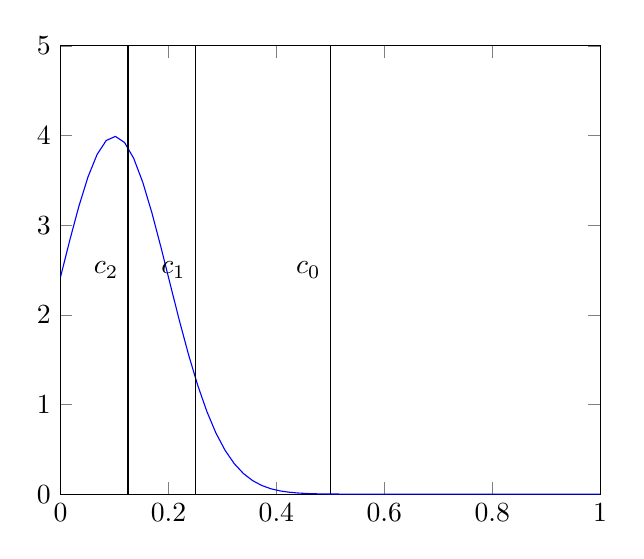
\begin{tikzpicture}
			\def\mean{0.1}
			\def\sigma{0.1}
			\def\pi{3.14159265359}
			\begin{axis}[xmin = 0, xmax = 1, ymin=0, ymax=5, samples=60]
				\addplot[domain = 0:1,blue] {1 / (\sigma * sqrt(2 * \pi)) * exp(-0.5 * ((x - \mean) / \sigma)^2) };
				\draw (axis cs:0.5,0) -- node[left]{$c_0$} (axis cs:0.5,5);
				\draw (axis cs:0.25,0) -- node[left]{$c_1$} (axis cs:0.25,5);
				\draw (axis cs:0.125,0) -- node[left]{$c_2$} (axis cs:0.125,5);
			\end{axis}
		\end{tikzpicture}
	\end{center}
	\caption{3 iterations of binary search with naive initial guess}\label{euclid}
\end{figure}

The underlying distribution is a normal distribution. \TODO{Add reference to section about data}. We can see that the algorithm will have to sweep 3 times over the entire array to get into the region of the actual median. One suggestion for improvement is to use an approximated median as a guess for the first split. We can sample 100 particles and find their median in constant time. Then we will run the binary cut algorithm using the approximated median as an initial guess. This can reduce the runtime by a few iterations, however we cannot make any assessment about the runtime, as this improvement will make the algorithm even slower on some distributions. Let us for example consider the uniform distribution, in this case the addition is pure overhead as the center is already the most accurate initial guess.
\end{comment}



\subsection{Reshuffling Algorithm}

\begin{algorithm}[H]
	\caption{Reshuffle algorithm}\label{euclid}
	\begin{algorithmic}[1]
		\Procedure{reshuffle}{$x, N_j, cut, axis$}
		\State $i = 0$
		
		\For{$k \in {0,..N_j - 1}$}
		\If{$\vec{x}_{k, axis} < split$}
		\State $i = i + 1$
		\State $x_{i}, x_{k} = x_{k}, x_{i}$
		\EndIf
		\EndFor
		
		\State $ x_{i}, x_{N_j-1} = x_{N_j-1}, x_{i}$
		\State \Return $i$
		\EndProcedure
	\end{algorithmic}
\end{algorithm}

The reshuffle algorithm has a clearly observable runtime of $O(N)$ since we iterate over all particles once. Since we need to touch each element at least once to reshuffle the entire array there is no better algorithm than this.


\vspace{5mm}

\newpage
\section{Theoretical Analysis of ORB runtime}

The nature of the ORB algorithm and its application with very large data-sizes, requires that we consider hardware for concrete implementation details. Since we do not have the time to empirically measure all viable option, we try to create a theoretical model. The algorithm is generally very heavy in memory access, but its operations are extremely simple. Therefore we need to consider not only benefits from increased parallelism in GPU hardware, but also possible speed-ups reached by generally higher bandwidths for GPU memory than CPU memory. On the other hand we need to mitigate the very low bandwidths between the GPU and CPU, which cannot be avoided altogether, as the data needs to be sent from the CPU to GPU before we can process it on the graphics processor.

In order to have a clear terminology and understanding of a computing system, we will briefly describe a general computer model which can be applied to most modern high performance systems.

A computing system consists of several nodes, where each node has one or more CPU`s and some additionally have one or more GPU`s. Both the CPU and the GPU have their own memory which are connected by a data link. The bandwidth of this link is called Memory Bandwidth. We name the capacity of the CPU Memory Bandwidth $B_{CPU}$ and the GPU Memory Bandwidth $B_{GPU}$. Furthermore we have a separate data link between the CPU and the GPU memory which is in some cases called PCI express, NVLink (for modern NVidia GPU`s) among others. We will referete to th ba $PCI$.

\Q{Why does summit use NVLink for CPU -> GPU comm?}

\begin{figure}[H]
	\begin{center}
		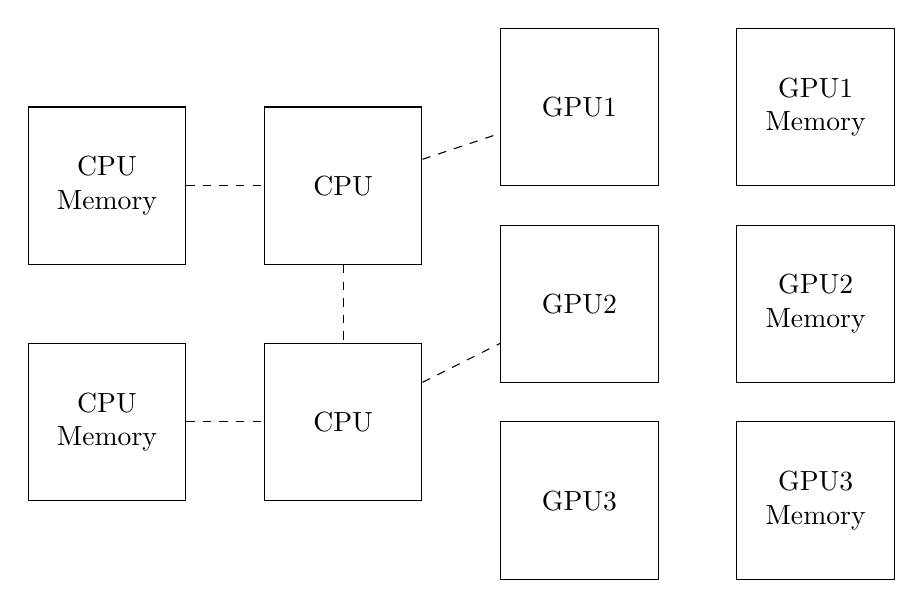
\begin{tikzpicture}
			
			\node[rectangle,
			draw = black,
			text = black,
			anchor = west,
			fill = white,
			align=center,
			minimum width = 2cm, 
			minimum height = 2cm] (cpu1) at (0cm,1.5cm) {CPU};
			
			\node[rectangle,
			draw = black,
			text = black,
			anchor = west,
			fill = white,
			align=center,
			minimum width = 2cm, 
			minimum height = 2cm] (cpu2) at (0cm,-1.5cm) {CPU};
			
			\node[rectangle,
			draw = black,
			text = black,
			anchor = west,
			fill = white,
			align=center,
			minimum width = 2cm, 
			minimum height = 2cm] (cpum1) at (-3cm,1.5cm) {CPU \\ Memory};
			
			\node[rectangle,
			draw = black,
			text = black,
			anchor = west,
			fill = white,
			align=center,
			minimum width = 2cm, 
			minimum height = 2cm] (cpum2) at (-3cm,-1.5cm) {CPU \\ Memory};
			
			\draw[dashed] (cpum1) to (cpu1);
			\draw[dashed] (cpum2) to (cpu2);
			\draw[dashed] (cpu1) to (cpu2);
			
			
			\node[rectangle,
			draw = black,
			text = black,
			anchor = west,
			fill = white,
			align=center,
			minimum width = 2cm, 
			minimum height = 2cm] (gpu1) at (3cm,2.5cm) {GPU1};
			
			\node[rectangle,
			draw = black,
			text = black,
			anchor = west,
			fill = white,
			align=center,
			minimum width = 2cm, 
			minimum height = 2cm] (gpu2) at (3cm,0cm) {GPU2};
			
			\node[rectangle,
			draw = black,
			text = black,
			anchor = west,
			fill = white,
			align=center,
			minimum width = 2cm, 
			minimum height = 2cm] (gpu3) at (3cm,-2.5cm) {GPU3};
			
				\node[rectangle,
			draw = black,
			text = black,
			anchor = west,
			fill = white,
			align=center,
			minimum width = 2cm, 
			minimum height = 2cm] (gpum1) at (6cm,2.5cm) {GPU1 \\ Memory};
			
			\node[rectangle,
			draw = black,
			text = black,
			anchor = west,
			fill = white,
			align=center,
			minimum width = 2cm, 
			minimum height = 2cm] (gpum2) at (6cm,0cm) {GPU2 \\ Memory};
			
			\node[rectangle,
			draw = black,
			text = black,
			anchor = west,
			fill = white,
			align=center,
			minimum width = 2cm, 
			minimum height = 2cm] (gpum3) at (6cm,-2.5cm) {GPU3 \\ Memory};
			
			
			\draw[dashed] (cpu1) to (gpu1);
			\draw[dashed] (cpu2) to (gpu2);
			\draw[dashed] (cpu1) to (cpu2);
			
		\end{tikzpicture}
	\end{center}
\end{figure}

We now sketch out various implementation ideas, derive for each a formula to estimate its runtime and finally insert datapoints from our target computing systems.
We assume that the data is stored in the CPU memory initially and we define the size of the data as $s$.

\TODO{Find tflops}

% Compare flops with speed of memory
% Add small experiment
% Memory Bandwidth Cliff
Let us assume a CPU with a clock speed of $cps$ per second. 

\subsection{Runtime estimations on a single node}

\TODO{Add introduction}
\TODO{Argue that is is similar on multinode systems as global reshuffling }


\TODO{Local partitioninig is not necessarily better, but simpler. }

\subsubsection{Naive implementation}

\begin{center}
	\begin{equation}
			p \times \frac{ s }{B_{CPU}} = t
			\label{eq:cpu}
	\end{equation}
\end{center}

\vspace{5mm}


The Equation \ref{eq:gpu} for the GPU is similar, the only difference being that we use the GPU memory bandwidth $B_{GPU}$ instead of the CPU bandwidth. Furthermore we have to consider the time it takes to send the data from the CPU to the GPU. This adds the terms size divided by CPU to GPU memory bandwidth denoted as $I$. Finally we also need to load the data from the CPU memory to the CPU before we are able to send it. 

\begin{center}
	\begin{equation}
		p \times \frac{s}{B_{GPU}} + \frac{s}{I}  + \frac{s}{B_{CPU}}= t
		\label{eq:gpu}
	\end{equation}
\end{center}

\vspace{5mm}


\subsubsection{GPU tree building}

Let us now consider an alternative way of computing binary cuts. We will build part of the tree on the GPU itself. This will allow us to reduce the very costly overheads imposed by transferring data from the CPU to the GPU. The maximum number of cuts we can perform is $p \times 3$. After p cuts we have $2^{p \times 3}$ leaf cells, and have reached the precision. Note that in this case we also need to send back the information about the built tree from the GPU to the CPU. 

\TODO{Too strong of a simplification}
\TODO{its log(d)}
\begin{center}
	\begin{equation}
		log(d) \times p \times \frac{s}{B_{CPU}} = t
		\label{eq:cputree}
	\end{equation}
\end{center}

\begin{center}
	\begin{equation}
		log(d) \times p \times \frac{s}{B_{GPU}} + 2 \times \frac{s}{I} = t
		\label{eq:gputree}
	\end{equation}
\end{center}


\subsubsection{Batch loading}

Finally we can also try to mitigate the overheads introduced by CPU to GPU communication by sending small batches, such that the GPU can already start processing the data, before the data transfer was completed. Lets denote the number of batches by $b$. For the sake of simplicity we only make a single cut and thus can reuse Equation \ref{eq:cpu} for the CPU version. For the GPU we now omit the term for memory access from the GPU. Because we can already start processing data in parallel when the first batch arrived and $B_{GPU} > I$ holds for every modern hardware. Thus the only overhead we still get is $\frac{s \div b}{B_{GPU}}$ for the very last batch, but as we can just increase b in relation to N, this becomes negligible. Note that this only counts for the very first iteration, thus the only difference we have is the constant of 31 and not 32. 

\begin{center}
	\begin{equation}
		(d-1) \times p \times \frac{s}{B_{GPU}} + 2 \times \frac{s}{I} = t
		\label{eq:gpubatch}
	\end{equation}
\end{center}

Due to possible overhead and no real improvement over the naive GPU version, we will omit the analysis using this method.

\subsubsection{Data compression}

Since for most computer the Interconnect bandwidth is greatly smaller than the Memory Bandwidth, we could potentially also think about compressing the particle data. This would increase computational costs, but would allow us to store a higher amount of particles and reduce the cost which comes from loading the particles from memory as well as sending the data over the Interconnect.

\begin{itemize}
	\item Why do we even use floats in the first place? wouldn't integers suit better since precision is uniformly equal?
	\item Reduce transfered number of bits, sacrifice precision?
\end{itemize}

\TODO{Add plots?}
\subsection{Datapoints of supercomputers}

We will compare the performance with the datapoints of Piz Daint, Summit and Alps which is a part of Eiger. We choose Piz Daint because we have the possibility to test the Code on its systems. We choose Eiger because we can also access its systems and it will give us a good reference values, due to it being a non hybrid supercomputer, meaning the nodes to not have GPU. Finally we analyze its performance on Summit, as its at the time of writing this thesis, one of the most capable supercomputers in the world.

\small
\begin{figure}[H]
	\begin{center}
		\begin{tabular}{ c c c c }
			& Piz Daint \cite{piz_daint} & Summit & Alps (Eiger) \\ 
			\hline
			Number of Nodes & 5704 & 4608 & 1024\\
			CPU Mem. Cap. & 64 GB & 256 GB $\times$ 2  \\   
			CPU Model & Intel E5-2690 v3 & IBM POWER9 $\times$ 2 & AMD EPYC 7742 \\
			CPU Mem. Bandw.  & 68 GB/s & 170 GB/s & 204.8 GB/s x 2	\\
			GPU Model & NVIDIA P100 & NVIDIA V100s  $\times$ 6 & None \\
			GPU Mem. Cap. & 16 GB & 16 GB $\times$ 6 & -\\
			GPU Mem. Bandw. & 732 GB/s & 900 GB/s & -\\
			Interconnect Bandw. & 32 GB/s & 50 GB/s & -\\
		\end{tabular}
	\end{center}
\caption{Datapoints of Supercomputers}
\label{fig:datapoints}
\end{figure}

We can now plug-in the values we obtained from different supercomputers in our equations.  We will assume a precision $p = 32$ bits which is sensible in the case of astrophysical simulations. \TODO{Add reference}.

\normalfont
\subsection{Piz Daint} 

Let us plugin the values from Figure \ref{fig:datapoints} into the corresponding formulas \ref{eq:cpu}, \ref{eq:gpu}, \ref{eq:cputree} and \ref{eq:gputree}.

\subsubsection{Naive implementation}
The naive implementation yields the following speeds for the naive CPU  implementation:

\pgfmathparse{32 * 12 / 68}

\begin{center}
	\begin{equation}
		32 \times \frac{ 12 GB }{68 GB/s} = \pgfmathresult s
	\end{equation}
\end{center}


And the corresponding GPU implementation:
\pgfmathparse{ 32 * 12 / 68}
\begin{center}
	\begin{equation}
		32 \times \frac{12 GB}{732 GB/s} + \frac{12 GB}{32 GB/s}  + \frac{12 GB}{68 GB/s} = 1.08s
	\end{equation}
\end{center}


%\begin{tikzpicture}
%	\begin{axis}[xmin = -1, xmax = 13, ymin=-1, ymax=6]
%		\addplot[domain = 0:12,blue] {(32 * x / 68) / (32 * x / 732 + x /32 + x/68) };
%	\end{axis}
%\end{tikzpicture}

This yields in a speed-up of:
\begin{center}
	\begin{equation}
		\frac{5.65s}{1.08} = 5.25
	\end{equation}
\end{center}


\subsubsection{GPU Tree Building}

\begin{center}
	\begin{equation}
		32 \times 32 \times \frac{ 12 GB }{68 GB/s} = 180s
	\end{equation}
\end{center}

And the corresponding GPU implementation:
\begin{center}
	\begin{equation}
		32 \times 32 \times \frac{12 GB}{732 GB/s} + 2 \times \frac{12 GB}{32 GB/s}  + \frac{12 GB}{68 GB/s} = 17.71s
	\end{equation}
\end{center}

This yields in a speed-up of:
\begin{center}
	\begin{equation}
		\frac{180s}{17.71} = 10.2
	\end{equation}
\end{center}

\vspace{5mm}


\subsection{Summit}

Let us plugin the values from Figure \ref{fig:datapoints} into the corresponding formulas \ref{eq:cpu}, \ref{eq:gpu}, \ref{eq:cputree} and \ref{eq:gputree}.

\subsubsection{Naive implementation}
The naive implementation yields the following speeds for the naive CPU  implementation:

\begin{center}
	\begin{equation}
		32 \times \frac{ 12 GB }{170 GB/s \times 2} = 2.56s
	\end{equation}
\end{center}

And the corresponding GPU implementation:
\begin{center}
	\begin{equation}
		32 \times \frac{12 GB}{900 GB/s \times 6} + \frac{12 GB}{50 GB/s \ times 6}  + \frac{12 GB}{170 GB/s \ times 2} = 0.74s
	\end{equation}
\end{center}

This yields in a speed-up of:
\begin{center}
	\begin{equation}
		\frac{2.56s}{0.74s} = 3.06
	\end{equation}
\end{center}


\subsubsection{GPU Tree Building}

\begin{center}
	\begin{equation}
		32 \times 32 \times \frac{ 12 GB }{170 GB/s} = 70.28s
	\end{equation}
\end{center}

And the corresponding GPU implementation:
\begin{center}
	\begin{equation}
		32 \times 32 \times \frac{12 GB}{900 GB/s} + 2 \times \frac{12 GB}{50 GB/s}  + \frac{12 GB}{170 GB/s} = 14.2s
	\end{equation}
\end{center}

This yields in a speed-up of:
\begin{center}
	\begin{equation}
		\frac{70.28s}{14.2s} = 4.95
	\end{equation}
\end{center}


\vspace{5mm}


\subsection{Eiger}

\begin{center}
	\begin{equation}
		32 \times 32 \times \frac{ 12 GB }{204.8 GB/s} = 60s
	\end{equation}
\end{center}

\subsection{Conclusion}

We conclude that the GPU version with GPU Tree building enabled yields the best speedup and also performs a lot better than the CPU version. Also we can observe that the speedup is bounded by $\frac{B_{GPU}}{B_{CPU}}$/ \TODO{Add reasoning}

\newpage
\section{Implementation}

\subsection{Data-structure}

\subsubsection{Tree}

The data-structure which stores the entire three needs to have following properties:

\begin{itemize}
	\item store domain information and provide access to left and right child cells
	\item Allow highly unbalanced trees
\end{itemize}

The most naive approach is to use a struct for each cell which stores information about the domain and keeps a pointer to the left and right cell. However since we in high performance systems, synchronizing pointers can be a bit of hassle, furthermore PKDGrav implements distributed arrays. Thus we can store all domain information in an array and simply keep track of the indices of its child cells. This can even be reduced further, since the right child cell is being created by the same process as the left child was. Thus we can assign the information about the right child in the positions left + 1 and only keep track of the index of the left child.

The minimal amount of data we need to store for each cell is its exact boundaries, the begin and end index in the particles array, and finally a index of the left child. If we sketch out two cells as a memory layout it looks as follows:
\begin{figure}[H]
	\begin{center}
		\begin{bytefield}{24}
			\begin{rightwordgroup}{cell 0}
				\memsection{0}{32}{2}{lower x}\\
				\memsection{32}{64}{2}{lower y}\\
				\memsection{64}{96}{2}{lower z}\\
				\memsection{96}{128}{2}{upper x}\\
				\memsection{128}{160}{2}{upper y}\\
				\memsection{160}{192}{2}{upper z}\\
				\memsection{192}{224}{2}{begin}\\
				\memsection{224}{256}{2}{end}\\
				\memsection{256}{288}{2}{left child}\\
			\end{rightwordgroup}\\
			\begin{rightwordgroup}{cell 1}
				\memsection{288}{320}{2}{lower x}\\
				\memsection{320}{352}{2}{lower y}\\
				\memsection{352}{384}{2}{lower z}\\
				\memsection{384}{416}{2}{upper x}\\
				\memsection{416}{448}{2}{upper y}\\
				\memsection{448}{480}{2}{upper z}\\
				\memsection{480}{512}{2}{begin}\\
				\memsection{512}{544}{2}{end}\\
				\memsection{544}{576}{2}{left child}\\
			\end{rightwordgroup}\\
			
		\end{bytefield}
	\end{center}
\end{figure}

Note that in theory we could only store the split position and axis for each particle, which would only require 32 bits for the positions and 2 bits (for 3D) for the axis. However the exact domain information can then only be achieved by traversing the three starting from the root. We can however make use of this data-structure when the communication overhead is greater than the costs of reconstructing the datastrucutre. Thus this storage version can be thought of as a lossless data compression of the tree.
\subsubsection{Particles}

The particles need to be stored in an array. We can implement the array using c style arrays, std::array or even an std::vector. The disadvantage of std::array and std::vector is their speed. On the other c-style arrays are limited in terms of multi dimensional indexing and boundary checking. Thus we make use of the library blitz++ which combines the speed of C-style arrays with the functionality of the std::vector. Furthermore blitz++ uses the same memory layout we would expect from a C-style array which looks as follows:

\begin{figure}[H]
	\begin{center}
		\begin{bytefield}{24}
			\begin{rightwordgroup}{particle 0}
				\memsection{0}{32}{4}{x}\\
				\memsection{32}{64}{4}{y}\\
				\memsection{64}{96}{4}{z}\\
			\end{rightwordgroup}\\
			\begin{rightwordgroup}{particle 1}
				\memsection{96}{128}{4}{x}\\
				\memsection{128}{160}{4}{y}\\
				\memsection{160}{192}{4}{z}\\
			\end{rightwordgroup}\\
		
		\end{bytefield}
	\end{center}
\end{figure}

\TODO{Data compression notice here?}


\subsection{Parallel Version Using Processes}

To parallelize the ORB algorithms, we first need to think about which parts of the algorithm can be parallelized and yield in a performance improvement. The most obvious choice for parallelization is the counting part from the binary cut algorithm. In this case the main thread (rank 0) will send a cut position and each processor counts how many particles there are on the left of this cut positions. It does so in a designated range of the entire particle array, which is unique to each rank.

\subsubsection{Local Reshuffling}

\begin{figure}[H]
	\begin{center}
		\begin{tikzpicture}
				
			\timeline{6}{16}{3}
			
			
			\parallelloop{-2}{15.5}{8}{0.5}{loop till all cells found};
		
			\parallelloop{-1}{11.5}{7}{3.5}{loop till cut found};
			
			\communication{Broadcast cells}{0}{7}{15};
						
			\process{local\\ reshuffle}{0}{14};
			\process{local\\ reshuffle}{2}{14};
			\process{local\\ reshuffle}{4}{14};
			\process{local\\ reshuffle}{6}{14};
			
			\process{compute\\ cut}{0}{11};
			
			 
			\communication{Broadcast cut from operative}{0}{7}{8};
			
			\process{local \\ count}{0}{7};
			\process{local \\ count}{2}{7};
			\process{local \\ count}{4}{7};
			\process{local \\ count}{6}{7};
	
			
			\communication{Reduce count to operative}{0}{7}{4};
			
			\process{generate\\ new \\ cells}{0}{3};

		\end{tikzpicture}
	\end{center}
\caption{Parallelized ORB for np = 4 and local reshuffling}
\label{fig:orb_parallel}
\end{figure}

\subsubsection{Global Reshuffling}

Another strategy we can use, as soon as we have created two domains, rank 0 can process one domain and rank 1 can process the other domain. This has the advantage that not only the counting part, but also the costly reshuffling part of the ORB algorithm can be parallelized. Furthermore the amount of data which needs to be communicated between the different threads is smaller. This is due to the fact that as soon as we found our first cut, only half the array of particles 


\begin{figure}[H]
	\begin{center}
		\begin{tikzpicture}
			
			\timeline{6}{8}{3}

			\communication{Compute cut}{0}{7}{7};
			\communication{Generate and Broadcast new cells}{0}{7}{6};
			
			\communication{Global reshuffle}{0}{7}{5};
			
			\communication{Compute cut}{0}{3}{4};
			\communication{Generate and \\ Broadcast new cells}{0}{3}{3};
			\communication{Global reshuffle}{0}{3}{2};
			
			\communication{Compute cut}{4}{7}{4};
			\communication{Generate and \\ Broadcast new cells}{4}{7}{3};
			\communication{Global reshuffle}{4}{7}{2};
			
			
		\end{tikzpicture}
	\end{center}
	\caption{Parallelized ORB for np = 4 and global reshuffling}
	\label{fig:orb_parallel}
\end{figure}

\TODO{Argue from communication standpoint. }

\vspace{5mm}

\subsubsection{Non parallelizable parts}
It is very difficult to parallelize the reshuffling part of the particle array. This is that it is very difficult to do in place. If we cannot perform it in place, we will probably have to use twice the memory capacity, which is will increase the maximum possible $N$ by a factor of two, which is not ideal.

\TODO{Extend section}

\subsection{Parallel Version Using CUDA }

\subsubsection{CUDA Memory Model}



% Use for reduction explanation https://texample.net/tikz/examples/database-decimation-process/
\bibliographystyle{plain}
\bibliography{reference}

\end{document}
